\documentclass[margin=2cm]{standalone}
%\usepackage{amssymb}		need this for \varnothing
\usepackage{tikz}
\usetikzlibrary{calc,intersections,through,backgrounds,patterns}

%Diagram showing equivalences between different fixpoint concepts used in economics
%Solid lines signify known results, dashed lines signify open problems
%Some of these open problems may have been solved since Zhao's paper, however.

%Zhao, J. (2002). ``The Equivalence between Four Economic Theorems and Brouwer’s Fixed Point Theorem.'' Working Paper. Retrieved from https://www.researchgate.net/publication/228432065_The_equivalence_between_four_economic_theorems_and_Brouwer%27s_fixed_point_theorem

\begin{document}

%\begin{figure}
%	\centering
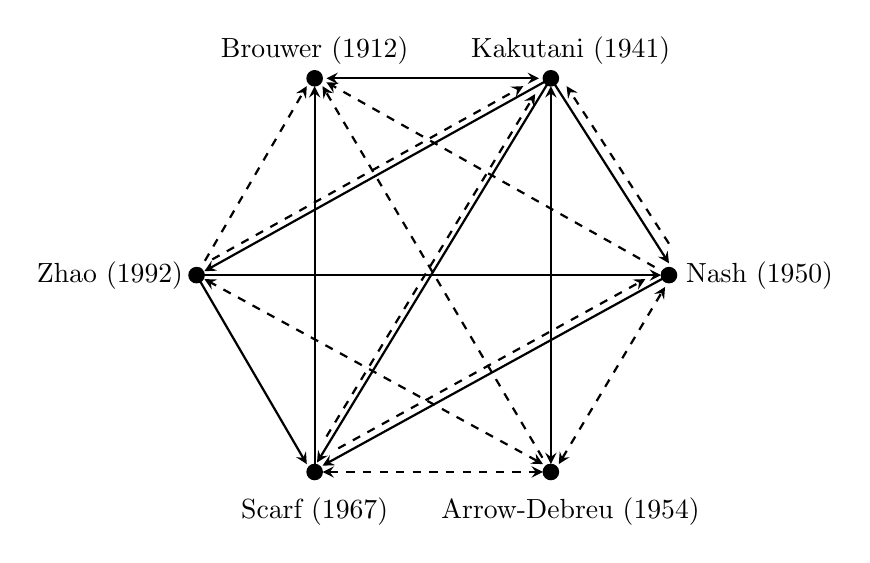
\begin{tikzpicture}[>=stealth]
\coordinate (S) at (0,0);
\coordinate (Z) at (-1.5,2.5);
\coordinate (B) at (0,5);
\coordinate (K) at (3,5);
\coordinate (A) at (3,0);
\coordinate (N) at (4.5,2.5);
\fill (S) circle (3pt);\fill (Z) circle (3pt);\fill (B) circle (3pt);
\fill (K) circle (3pt);\fill (A) circle (3pt);\fill (N) circle (3pt);

%outer lines
\draw [<->, thick] 		   (0.15,5)--(2.85,5);	 %B--K
\draw [->, thick, dashed]  (Z)--(-0.1,4.9);		 %Z--B
\draw [->, thick] 		   (Z)--(-0.1,0.1);		 %Z--S
\draw [<->, thick, dashed] (0.1,0)--(2.9,0);	 %S--A
\draw [<->, thick, dashed] (3.1,0.1)--(4.45,2.35); %A--N
\draw [->, thick] 		   (K)--(4.5,2.65);		 %K--N

%middle lines, horizontal & vertical
\draw [->, thick] (-1.5,2.5)--(4.4,2.5);	%Z--N
\draw [->, thick] (S)--(0,4.9);				%S--B
\draw [<->, thick] (3,0.1)--(3,4.9);		%K--A

%middle lines, diagonal
\draw [->, thick]  		   (K)--(-1.4,2.55);	  %K--Z
\draw [->, thick] 		   (K)--(0.03,0.12);	  %K--S
\draw [->, thick]		   (N)--(0.1,0.08);		  %N--S
\draw [->, thick, dashed]  (N)--(0.15,4.95);	  %N--B
\draw [->, thick, dashed]  (A)--(0.1,4.9);		  %A--B
\draw [<->, thick, dashed] (2.9,0.1)--(-1.4,2.45);%A--Z

%middle lines, diagonal, secondary
\draw [->, thick, dashed]  (-1.3,2.7)--(2.65,4.9);		%Z--K
\draw [->, thick, dashed]  (0.15,0.45)--(2.8,4.8);		%S--K
\draw [->, thick, dashed]  (4.5,2.9)--(3.2,4.9);		%N--K
\draw [->, thick, dashed]  (0.3,0.3)--(4.2,2.45);		%S--N

%labels
\node at (-2.6,2.5)  {Zhao (1992)};
\node at (0,5.35)  	 {Brouwer (1912)};
\node at (0,-0.5) 	 {Scarf (1967)};
\node at (3.25,-0.5) {Arrow-Debreu (1954)};
\node at (5.65,2.5)  {Nash (1950)};
\node at (3.25,5.35) {Kakutani (1941)};

\end{tikzpicture}
%	\caption{The equivalence between Brouwer's or Kakutani's fixed point theorem and the existence theorems of Nash equilibrium, competitive equilibrium, core and hybrid solution.}
%\end{figure}

\end{document}